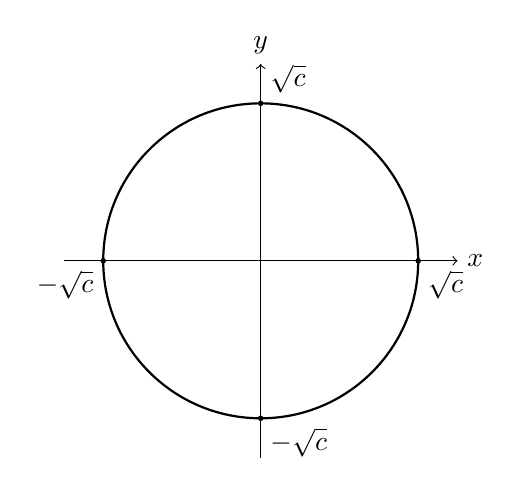
\begin{tikzpicture}[scale=1]

  % Definir el radio
  \def\r{2} % aquí puedes cambiar el valor (esto representa \sqrt{c})

  % Ejes
  \draw[->] (-\r-0.5,0) -- (\r+0.5,0) node[right] {$x$};
  \draw[->] (0,-\r-0.5) -- (0,\r+0.5) node[above] {$y$};

  % Circunferencia
  \draw[thick] (0,0) circle (\r);

  % Puntos de intersección con los ejes
  \fill (\r,0) circle (1pt) node[below right] {$\sqrt{c}$};
  \fill (-\r,0) circle (1pt) node[below left] {$-\sqrt{c}$};
  \fill (0,\r) circle (1pt) node[above right] {$\sqrt{c}$};
  \fill (0,-\r) circle (1pt) node[below right] {$-\sqrt{c}$};

\end{tikzpicture}

